\section{Parallel coordinate descent methods}\label{pcdm}
We demonstrated that the true $PSF$ of the deconvolution problem can be approximated. A smaller $PSF$ can be used, which is only a fraction of the true size. The serial coordinate descent methods, which was used so during this project, achieves a moderate speedup with the $PSF$ approximation. Parallel coordinate descent methods may benefit more from the $PSF$ approximation. For the rest of this work, we develop a parallel coordinate descent deconvolution algorithm. We explain why parallel methods should benefit more from the $PSF$ approximation, and show that they indeed speed up the deconvolution problem.


Introduce the principle of parallel coordinate descent methods, and derrive a parallel coordinate descent deconvolution algorithm.

%Naive way to exploit this, we can create patches of the image, four of which are independent of each other.
%Deconvolve four patches in parallel.
%Work is not equally distributed on the different patches. 



\subsection{From serial to parallel}
Parallel coordinate descent methods take several steps at different coordinates before they update the gradient map. The difficulty in parallel coordinate descent methods lies in dealing with correlated pixel values> In our deconvolution problem, two pixels which are close to each other in the image are correlated. The more they overlap, the more we over-estimate their pixel values with parallel coordinate descent methods\footnote{Imagine we optimize two pixels next to each other in serial coordinate descent: The serial coordinate descent algorithm  optimizes he first pixel, updates the gradient, and then optimizes the second pixel. The value of the second pixel will be magnitudes lower than the first, because most of the emission in that area was already explained by the first pixel. If however we update in parallel, both pixels will end up with a similar value, and both pixels try to explain the same emission.}. This over-estimation leads to slow convergence. Or if we increase the number of parallel updates, can lead to a divergence. This means we cannot simply modify our serial coordinate descent algorithm to take a number of parallel steps. We need a way to deal with the over-estimation. 

Our serial coordinate descent algorithm uses a greedy pixel selection strategy. Parallel coordinate descent methods on the other hand often select their pixels uniformly at random. The random selection strategy lets us estimate how much the parallel algorithm over-estimates the pixel values\cite{richtarik2016parallel}. However, a random strategy is not efficient for our deconvolution problem.

We first explain the parallel coordinate descent method in the next section \ref{pcdm:pcdm}. We then introduce the modifications we developed for an efficient parallel deconvolution algorithm.

%Parallel coordinate descent methods have a strategy to deal with correlated pixel values: The shotgun algorithm\cite{bradley2011parallel} estimates the number parallel random updates that can be taken without diverging. PCDM estimates the expected $PSF$ overlap between random pixels, and adjusts the step size accordingly. In this project, we use the PCDM algorithm and its accelerated variant APPROX \cite{fercoq2015accelerated}. We introduce the algorithm in Section \ref{pcdm:pcdm}.

%Note that parallel coordinate descent methods tend to select pixels at random. This helps dealing with correlated pixel values: In our deconvolution case, the pixels which are close by to each other tend to be correlated more strongly. But the exact shape of the $PSF$ is also a factor. If the $PSF$s overlap only in a region where it is close to zero, the pair of pixels also have a low correlation factor. A random selection strategy helps to keep a low correlation factor on average, no matter what the $PSF$ looks like. 

%But for our deconvolution case, a random strategy brings in its own issues. Remember that the LMC has a bright supernova remnant N132D, which overshadows other sources. A deconvolution algorithm has to deconvolve the pixels belonging to N132D first. A random strategy may waste resources until it has deconvolved the fairly small subset of pixels belonging to N132D. We have adapted the PCDM algorithm for the deconvolution problem, and describe our adaption in detail in Section  \ref{pcdm:adaption}.

\subsection{Parallel (Block) Coordinate Descent Method (PCDM)} \label{pcdm:pcdm}
The PCDM algorithm can be seen as a generalization of our serial coordinate descent algorithm from Section \ref{cd}. The serial algorithm optimizes a single pixel at a time. PCDM can update one, or a whole block of pixels at each iteration. And as the name implies, it can update multiple blocks of pixels in parallel. In this project, we use the accelerated variant of the PCDM algorithm, named APPROX \cite{fercoq2015accelerated}. We first introduce a PCDM deconvolution algorithm and then describe the accelerated variant.

\subsubsection{Serial block coordinate descent deconvolution}
Here we introduce the serial block coordinate descent algorithm. Instead of optimizing a single pixel in each iteration, the serial block coordinate descent algorithm can update a block of pixels. The block size is left for the user to define. It can be any number between a single pixel, in which case the algorithm is identical to the serial coordinate descent algorithm from Section \ref{cd}, or the whole image.

Remember the single pixel update from the serial coordinate descent algorithm: 
\begin{equation} \label{pcdm:pcdm:block:single:update}
pixel_{opt} = \frac{max(gradient_{location} - \lambda\alpha, 0)}{Lipschitz_{location} + (1 - \alpha)\lambda}
\end{equation}

We optimize the pixel at the current location by taking the gradient and dividing it by the Lipschitz constant. For the serial block coordinate descent algorithm we vectorize the update rule. That means $gradient_{location}$ and $Lipschitz_{location}$ and the output $pixel_{opt}$ become vectors:

\begin{equation} \label{pcdm:pcdm:block:block:update}
pixels_{opt} = \frac{max(gradients_{locations} - \lambda\alpha, 0)}{Sum(Lipschitz_{locations}) + (1 - \alpha)\lambda}
\end{equation}

This is the serial block coordinate descent update rule. Note that we divide the gradient for each pixel by the the block Lipschitz constant (which is the sum of every pixel Lipschitz constant in the block). The single pixel update rule can take a larger step, but only for a single pixel. 

The reader might be familiar with the (F)ISTA method\cite{beck2009fista}. The block update shown in equation \eqref{pcdm:pcdm:block:block:update} is related to the (F)ISTA update step. When the block size equal to the image size (we update all pixels in the image in each iteration), then the serial block coordinate descent is equivalent to (F)ISTA.


\subsubsection{Parallel block coordinate descent deconvolution}
We present the parallel block coordinate descent algorithm. It is based on the PCD method\cite{richtarik2016parallel}. In this section, we show how it can be used to solve the deconvolution problem. Our parallel coordinate descent algorithm updates $t$ random blocks of pixels in parallel in each iteration. Each iteration is split into three steps: Step 1 is to select $t$ unique blocks of pixels uniformly at random (we cannot select the same block multiple times). In step 2 we update in parallel each selected block in the reconstructed image $x$. And finally in step 3 we update the gradient map.

\begin{lstlisting}
dirty = IFFT(GridVisibilities(visibilities))
residualsPadded = ZeroPadding(dirty)

psfPadded = ZeroPadding(PSF)
psfPadded = FlipUD(FlipLR(psfPadded))
gradientUpdate = iFFT(FFT(ZeroPadding(PSF)) * FFT(psfPadded))

x = new Array[,]
gradientsMap = iFFT(FFT(residualsPadded) * FFT(psfPadded))
lipschitzMap = CalcLipschitz(PSF)

objectiveValue = 0.5* Sum(residuals * residuals) + ElasticNet(x)
eso = ESO(CountNonZero(PSF), t, x.Length / blockSize)

do 
	oldObjectiveValue = objectiveValue
	
	//Step 1: select t blocks uniformly at random
	blocks = sample(t)
	
	//Step 2: update reconstruction
	diffBlocks = new Array
	parallel for each block in blocks
		blockLipschitz = Sum(GetBlock(LipschitzMap, block))
		
		//increase blockLipschitz according to the ESO
		blockLipschitz = blockLipschitz * eso
		gradientsBlock = GetBlock(gradientMap, block)
		oldBlock = GetBLock(x, block)
		tmp = gradientsBlock + oldBlock * blockLipschitz
		optimalBlock = Max(tmp - lambda*alpha) / (blockLipschitz + (1 - alpha)*lambda)
		diffBlock = optimalBlock - oldBlock
		
		x[block] += diffBlock
		diffBlocks[block] = diffBlock
	
	//Step 3: Update gradients
	for each block in blocks
		diffBlock = diffBlocks[block]
		for each pixel in block
			diff = diffBlock[pixel]
			shiftedUpdate = Shift(gradientUpdate, pixelLocation)
			gradientMap = gradientMap - shiftedUpdate * diff
			
while maxAbsDiff  < epsilon
\end{lstlisting}

The parameter $t$ can be thought of as the number of processors. We select a block to optimize in parallel for each available processor. The parallel algorithm presented here is a synchronous implementation. Each processor waits for the others to finish in each step. The implementation used later in this section is asynchronous, where each processor separately selects a block, updates the reconstruction and updates the gradient map independent of the other processors. 

Asynchronous implementation with compare exchange. gradient map gets updated asynchronously.

The core of the parallel coordinate descent algorithm is the Estimated Seperability Overapproximation (ESO). In essence, the ESO represents how much we over-estimate the pixels values when we update $t$ random blocks in parallel. To guarantee convergence, we decrease the step size by the factor of the ESO. With more processors $t$ involved, we have to take smaller and smaller steps to guarantee convergence. Here is a trade-off between the degree of parallelism and the overall convergence speed.

The ESO is derived from three components: The uniform sampling strategy used, the number of parallel updates, and the number of non-zero components in the $PSF$. We use a $t$-nice uniform sampling. The ESO that arises from the $t$-nice sampling (take $t$ blocks uniformly at random) according to\cite{richtarik2016parallel}:

\begin{equation}\label{pcdm:pcdm:eso}
ESO(\omega, t, n) = 1+ \frac{(\omega - 1)(t - 1)}{max(1, n -1)}
\end{equation}

Where $\omega$ is the number of non-zero entries in the $PSF$, $t$ is the number of parallel updates, and $n$ is the number of blocks in the problem. For example: The image is $256^2$ pixels in size, we update blocks with a size of $4^2$ pixels, the $PSF$ has $\omega = 24$ non zero entries, and we use $t = 4$ processors, then the ESO is:

\begin{equation}
ESO(\omega = 24, t = 4, n = (256^2 / 4^2)) = 1+ \frac{(24 - 1)(4 - 1)}{max(1, 4096 -1)} \approx 1.017
\end{equation}

The lowest possible value for the ESO is $1$. The fewer processors $t$ we use and the fewer non-zero components $\omega$ the $PSF$ has, the closer the ESO is to 1. We want a small ESO with the highest number of processors possible. As we see from equation \eqref{pcdm:pcdm:eso}, the ESO gets smaller with fewer non-zero values in the $PSF$.

Remember that the $PSF$ in radio astronomy is typically dense. Although most of its values are close to zero, it generally does not have any zero values. The $PSF$ approximation methods we developed in Section \ref{gradient} effectively reduce the number of non-zero values. For the parallel coordinate descent algorithm, this leads to an ESO closer to 1, even  and we can take larger steps without diverging.


\subsection{Accelerated parallel block coordinate descent method}
We introduced the parallel coordinate descent algorithm in the previous section. In this section we extend the previous algorithm with gradient acceleration, similar to the APPROX method \cite{fercoq2015accelerated}.

Instead of using a single gradient map and a single reconstructed image $x$ variable, we an 'explore' and 'correction' variable of both. The algorithm uses an $xExplore$,  $xCorrection$ and $gradientMapExplore$, $gradientMapCorrection$. Intuitively, the 'correction' variables contain the accelerated part of the algorithm, and the 'explore' variables the standard part.

We introduce the acceleration variable $theta$, and arrive at the following accelerated, parallel block coordinate descent algorithm:
\begin{lstlisting}
dirty = IFFT(GridVisibilities(visibilities))
residualsPadded = ZeroPadding(dirty)

psfPadded = ZeroPadding(PSF)
psfPadded = FlipUD(FlipLR(psfPadded))
gradientUpdate = iFFT(FFT(ZeroPadding(PSF)) * FFT(psfPadded))

xExplore = new Array[,]
xCorrection = new Array[,]
gradientsMapExplore = iFFT(FFT(residualsPadded) * FFT(psfPadded))
gradientMapCorrection = new Array[,]
lipschitzMap = CalcLipschitz(PSF)

objectiveValue = 0.5* Sum(residuals * residuals) + ElasticNet(x)
eso = ESO(CountNonZero(PSF), t, x.Length / blockSize)
theta0 = t / (x.Length / blockSize)
theta = theta0

do 
	oldObjectiveValue = objectiveValue
	
	//Step 1: select t blocks uniformly at random
	blocks = sample(t)
	
	//Step 2: update reconstruction
	diffBlocks = new Array
	parallel for each block in blocks
	blockLipschitz = Sum(GetBlock(LipschitzMap, block))
	
	//increase blockLipschitz according to the ESO
	blockLipschitz = blockLipschitz * eso
	oldBlock = 
	tmp = theta^2 * GetBlock(gradientsMapCorrection, block) + GetBlock(gradientsMapExplore, block) + GetBLock(xExplore, block) * blockLipschitz
	optimalBlock = Max(tmp - lambda*alpha) / (blockLipschitz + (1 - alpha)*lambda)
	diffBlock = optimalBlock - oldBlock
	
	xExplore[block] += diffBlock
	xCorrection[block] += diffBlock * (-(1.0f - theta / theta0) / theta^2)
	diffBlocks[block] = diffBlock
	
	//Step 3: Update gradients
	for each block in blocks
		diffBlock = diffBlocks[block]
		for each pixel in block
			diff = diffBlock[pixel]
			shiftedUpdate = Shift(gradientUpdate, pixelLocation)
			
			gradientsMapExplore = gradientsMapExplore - shiftedUpdate * diff
			gradientsMapCorrection = gradientsMapCorrection - shiftedUpdate * diff * (-(1.0f - theta / theta0) / theta^2);
			
	theta = (Sqrt((theta^2 * theta^2) + 4 * (theta^2)) - theta^2) / 2.0f;

while maxAbsDiff  < epsilon

output = new float[,]
for(i in in Range(0, dirty.Length(0))
	for(j in in Range(0, dirty.Length(0))
	output[i, j] = theta * xCorrection[i, j] + xExplore[i, j];
\end{lstlisting}

The accelerated variant takes larger steps towards the optimum during deconvolution. As such, it should need fewer iterations to converge than the non-accelerated variant. Note that the accelerated deconvolution algorithm reduces to the normal parallel deconvolution algorithm if we skip the $theta$ update. Then, the 'correction' variables stay zero over all iterations.

The acceleration comes with a cost attached: Instead of a single gradient map and a single reconstructed image, the acceleration algorithm updates two of each. It is not clear whether the added costs of maintaining the 'explore' and 'correction' variables outweigh the benefit we receive with acceleration. As we will see later, the non-accelerated variant is actually faster on the LMC observation than the accelerated variant.


\subsection{The problem with random selection for deconvolution} \label{pcdm:adaption}
Both algorithms, the accelerated and non-accelerated variant as presented here do not perform well on the LMC dataset. The reason lies in the random selection strategy: In the first few iterations, the deconvolution algorithm selects blocks at random, and tries to explain the whole emission in that area. In short, the first iterations always over-estimate the block-values. 

\begin{figure}[h]
		\centering
	\begin{subfigure}[b]{0.245\linewidth}
		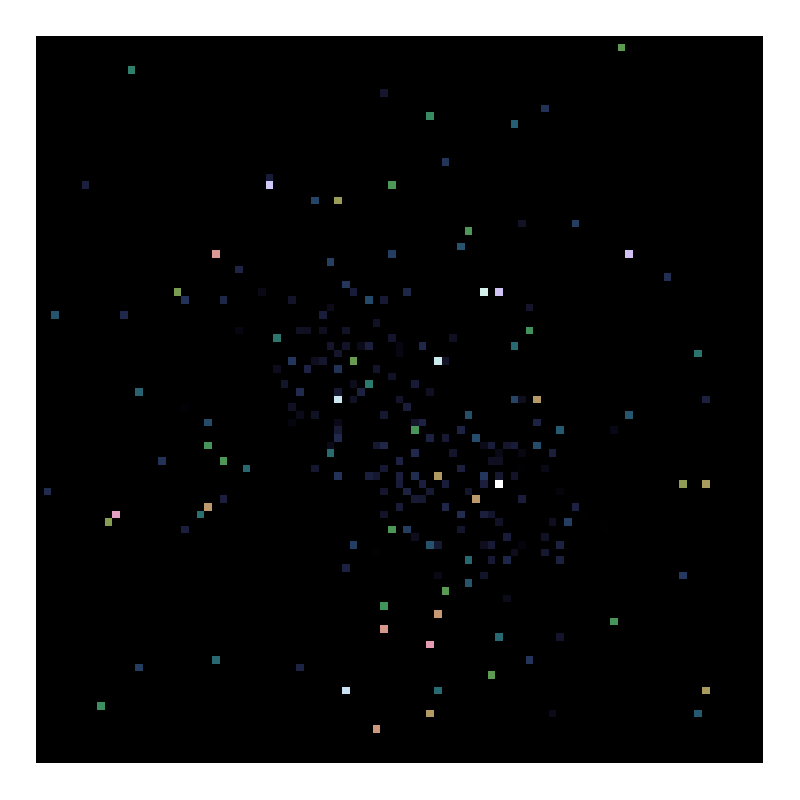
\includegraphics[width=1.00\linewidth, clip, trim= 0.25in 0.25in 0.25in 0.25in]{./chapters/05.pcdm/randomProblem/random_1k_block1.png}
		\caption{8k iterations}
		\label{pcdm:adaption:randomProblem:block11}
	\end{subfigure}
	\begin{subfigure}[b]{0.245\linewidth}
		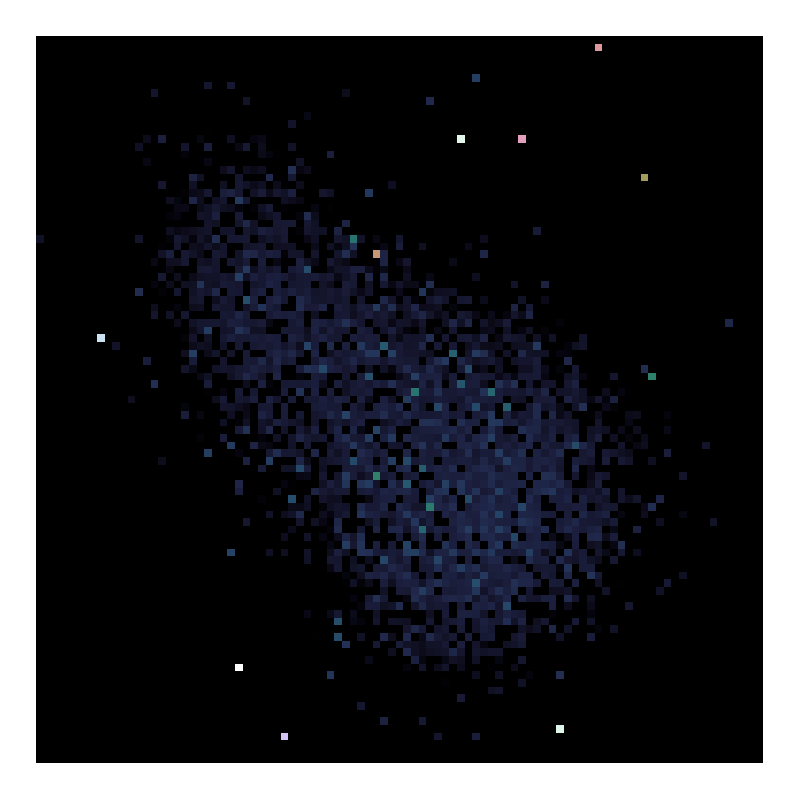
\includegraphics[width=1.00\linewidth, clip, trim= 0.25in 0.25in 0.25in 0.25in]{./chapters/05.pcdm/randomProblem/random_10k_block1.png}
		\caption{80k iterations}
		\label{pcdm:adaption:randomProblem:block12}
	\end{subfigure}
		\begin{subfigure}[b]{0.245\linewidth}
		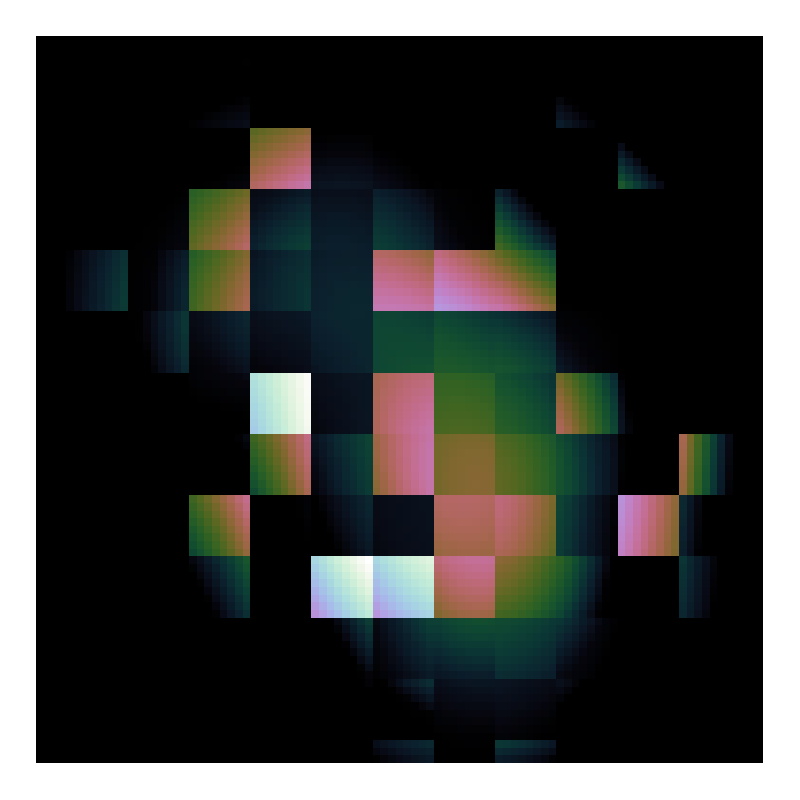
\includegraphics[width=1.00\linewidth, clip, trim= 0.25in 0.25in 0.25in 0.25in]{./chapters/05.pcdm/randomProblem/random_1k_block8.png}
		\caption{8k iterations, $8^2$ block}
		\label{pcdm:adaption:randomProblem:block81}
	\end{subfigure}
		\begin{subfigure}[b]{0.2405\linewidth}
		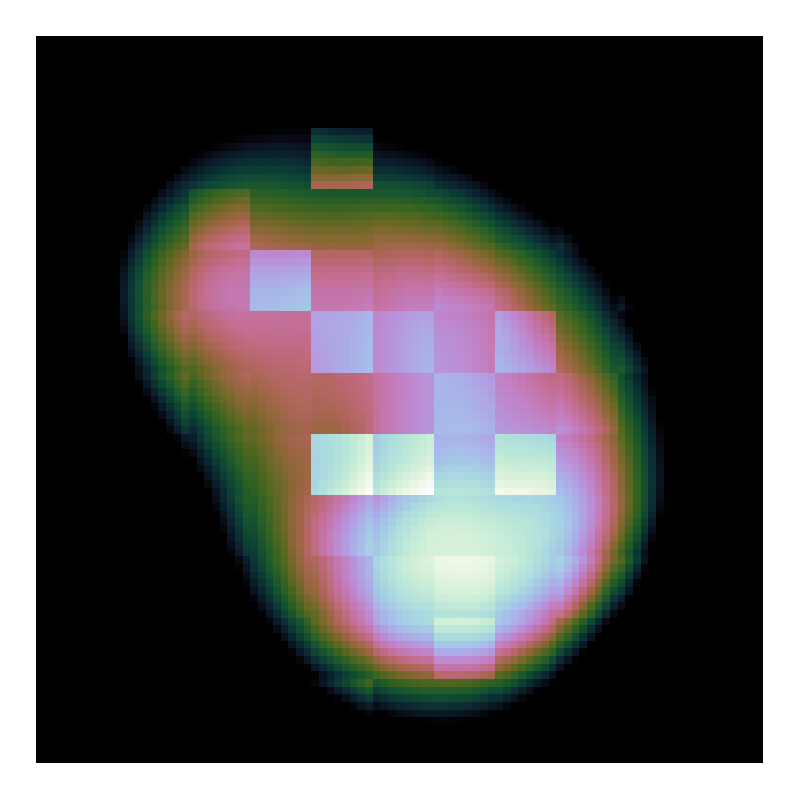
\includegraphics[width=1.00\linewidth, clip, trim= 0.25in 0.25in 0.25in 0.25in]{./chapters/05.pcdm/randomProblem/random_10k_block8.png}
		\caption{80k iterations, $8^2$ block}
		\label{pcdm:adaption:randomProblem:block82}
	\end{subfigure}
	\caption{Random parallel deconvolutions on the LMC N132D supernova remnant.}
	\label{pcdm:adaption:randomProblem}
\end{figure}

The Figure \ref{pcdm:adaption:randomProblem} shows the behaviour on the LMC observation. The reconstructions receive obvious artifacts from the random selection strategy. The blocks, which get selected in the first few iterations, keep their over-estimated values until we randomly select them again in later iterations. Other blocks in the neighborhood cannot be changed to a reasonable value until the algorithm has randomly selected the over-estimated blocks. That is why even after 80k iterations, the N132D supernova remnant gets only hinted at in Figure \ref{pcdm:adaption:randomProblem:block12}. Until the over-estimated blocks get selected again, the algorithm cannot do useful updates in that region.

This behavior is pronounced when we choose a block size of one pixel (i.e. we do not group pixels into blocks). Increasing the block size also increases our changes to select one of the over-estimated block again. But as we see in Figure \ref{pcdm:adaption:randomProblem:block82}, the same problem exists with larger block sizes, although less pronounced. After 80k iterations the N132D supernova remnant is visible, but a few random blocks still contain too much of the emission in that area.

The order in which we select blocks seems to be relevant in the deconvolution problem. A random selection strategy needs a prohibitive large number of iterations to converge. But we cannot simply switch out the selection strategy. The random selection strategy is at the core of the Parallel coordinate descent methods. Remember the ESO arises from the fact that we select $tau$ pixels uniformly at random. When we select $tau$-pixels with a greedy strategy, we might break the ESO and may not converge.

To solve this behavior, we introduce the pseudo-random selection strategy:  We select a block at random, but greedily search in the neighborhood for the optimal block to optimize. The size of the neighborhood can be defined by the user. It is essentially a mix between a greedy and a random selection strategy. If we choose the neighborhood to be the whole image, we arrive at a greedy strategy. If we choose the neighborhood to be just one block, we are back at a random strategy. The mixture of the greedy and random strategy allows us to fix the problems with the pure random

We also introduced three heuristics that speed up the parallel deconvolution algorithm in practice: An active set heuristic, Restarting heuristic and a 'Minor' cycle.


\subsubsection{Active set heuristic}
The active set heuristic is typically used in cyclic coordinate descent: It chooses a subset of blocks, and optimizes the set until it converges. Then it chooses a  new set. We use the active set heuristic together with our pseudo-random selection strategy. A large portion of the blocks in the image will be zero. If we select blocks at pseudo-random, we are likely to select a block that will never contain non-zero values. The active set heuristic increases the likelihood that the pseudo-random strategy selects a relevant block. 

At the start of the parallel deconvolution algorithm, we iterate over all blocks. We add all blocks whose value can be changed to non-zero. During parallel iterations, the algorithm only selects blocks from the active set.




\subsubsection{Restarting heuristic}
In accelerated gradient methods, like APPROX or (F)ISTA, restarting the acceleration can lead to a significant speedup\cite{fercoq2016restarting}.

Can improve convergence speed a lot.

Show code

In our case, we need to change the active set more often. Basically need to restart the acceleration parameter $\theta$ each time we change the active set.


\subsubsection{'Minor' cycles}
PSF approximations work really well.
Then we need more major cycles, which kill the benefit from the $PSF$ approximation

How far we can go with the approximation and the current dirty image.
Re-introduce something similar to the minor cycle of CLEAN. We start the minor cycle by deconvolving the dirty image with the approximate $PSF$. The residuals are now only an approximation, since we used the smaller $PSF$. We now reset the residuals, we convovle the full $PSF$ with the reconstructed image and subtract the result from the dirty image.

We can skip some major cycles.


\subsection{Tests on the LMC Observation}
Does the parallel deconvolution algorithm benefit more from the $PSF$ approximation?

Our heuristics have several parameters, we do a sweep on them and see what happens

What was tested
Just the pure active set iterations. Boiler plate code was not tested

We measure the time and the objective value. What parameters lead to the fastest convergence times.


\subsubsection{$PSF$ approximation}
We expect to benefit a lot more

Use the combined $PSF$ approximation.
\begin{figure}[h]
	\centering
	\begin{subfigure}{0.6\linewidth}
		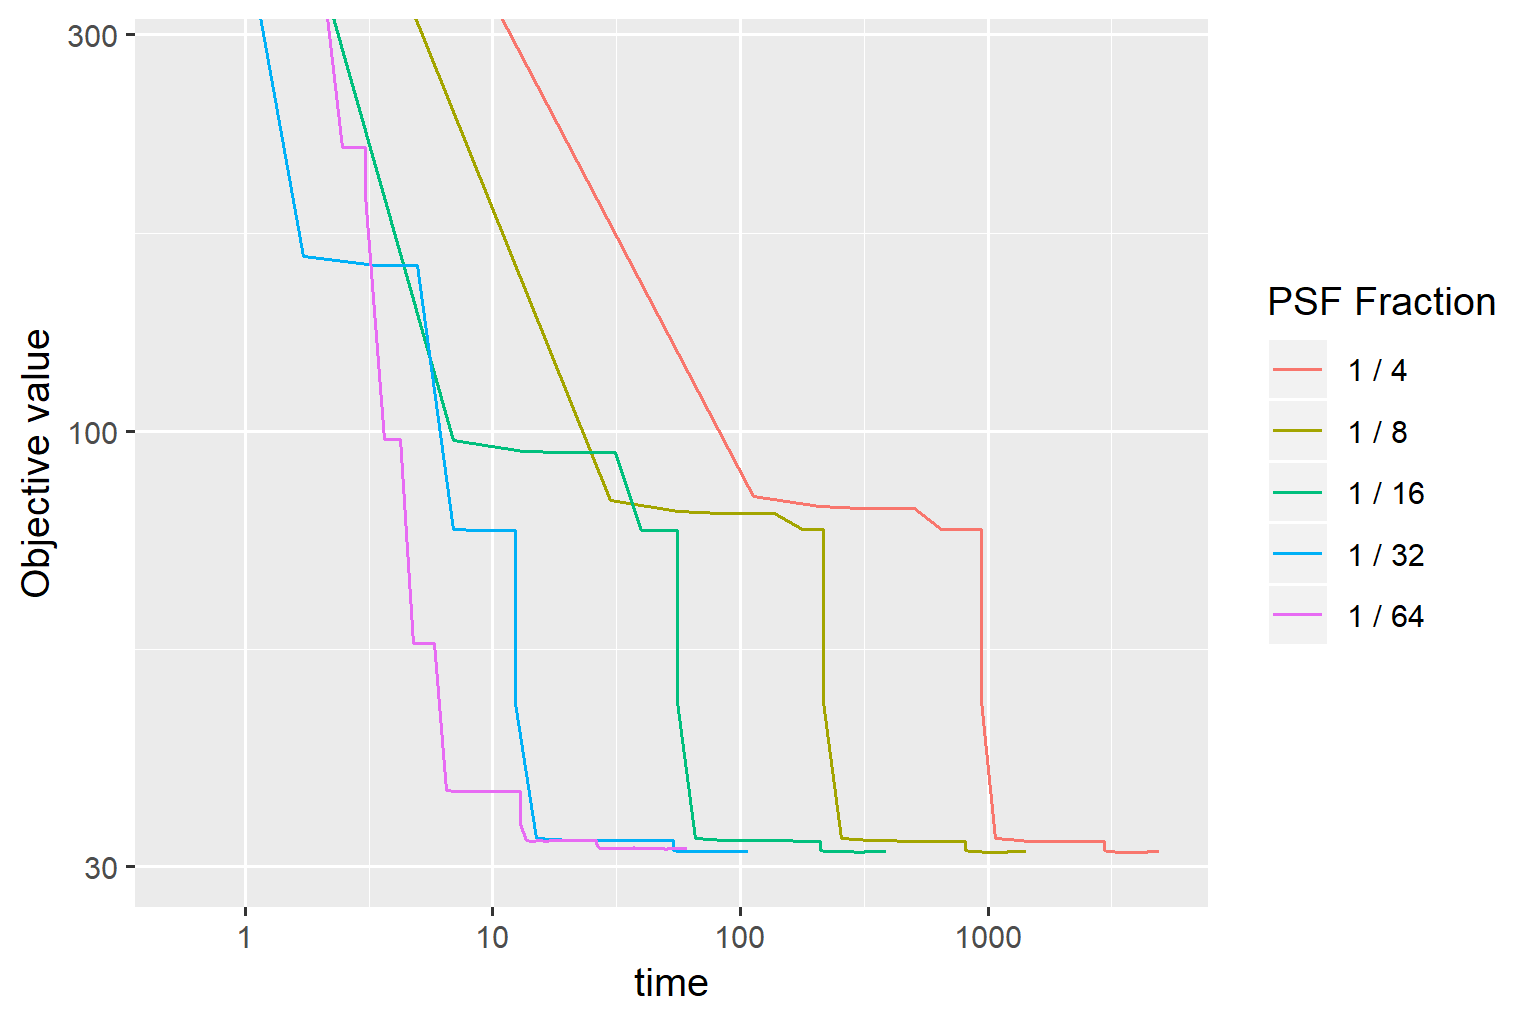
\includegraphics[width=1.0\linewidth]{./chapters/05.pcdm/parameters/psfSize.png}
	\end{subfigure}
	\begin{subfigure}{0.35\linewidth}
		\begin{tabular}{c | c}
			PSF Fraction & Total seconds \\ \hline
			1 / 4 & 4941 \\
			1 / 8 & 1433 \\
			1 / 16 & 390 \\
			1 / 32 & 108 \\
			1 / 64 & 61 \\
		\end{tabular}
	\end{subfigure}
	\caption{Convergence speedup with $PSF$ approximation}
\end{figure}

And it does. A clear advantage for using. Large speedup factor
Question whether to use $\frac{1}{32}$ or $\frac{1}{64}$.


\subsubsection{Block size}
Test the effect of increasing the block size

\begin{figure}[h]
	\centering
	\begin{subfigure}{0.6\linewidth}
		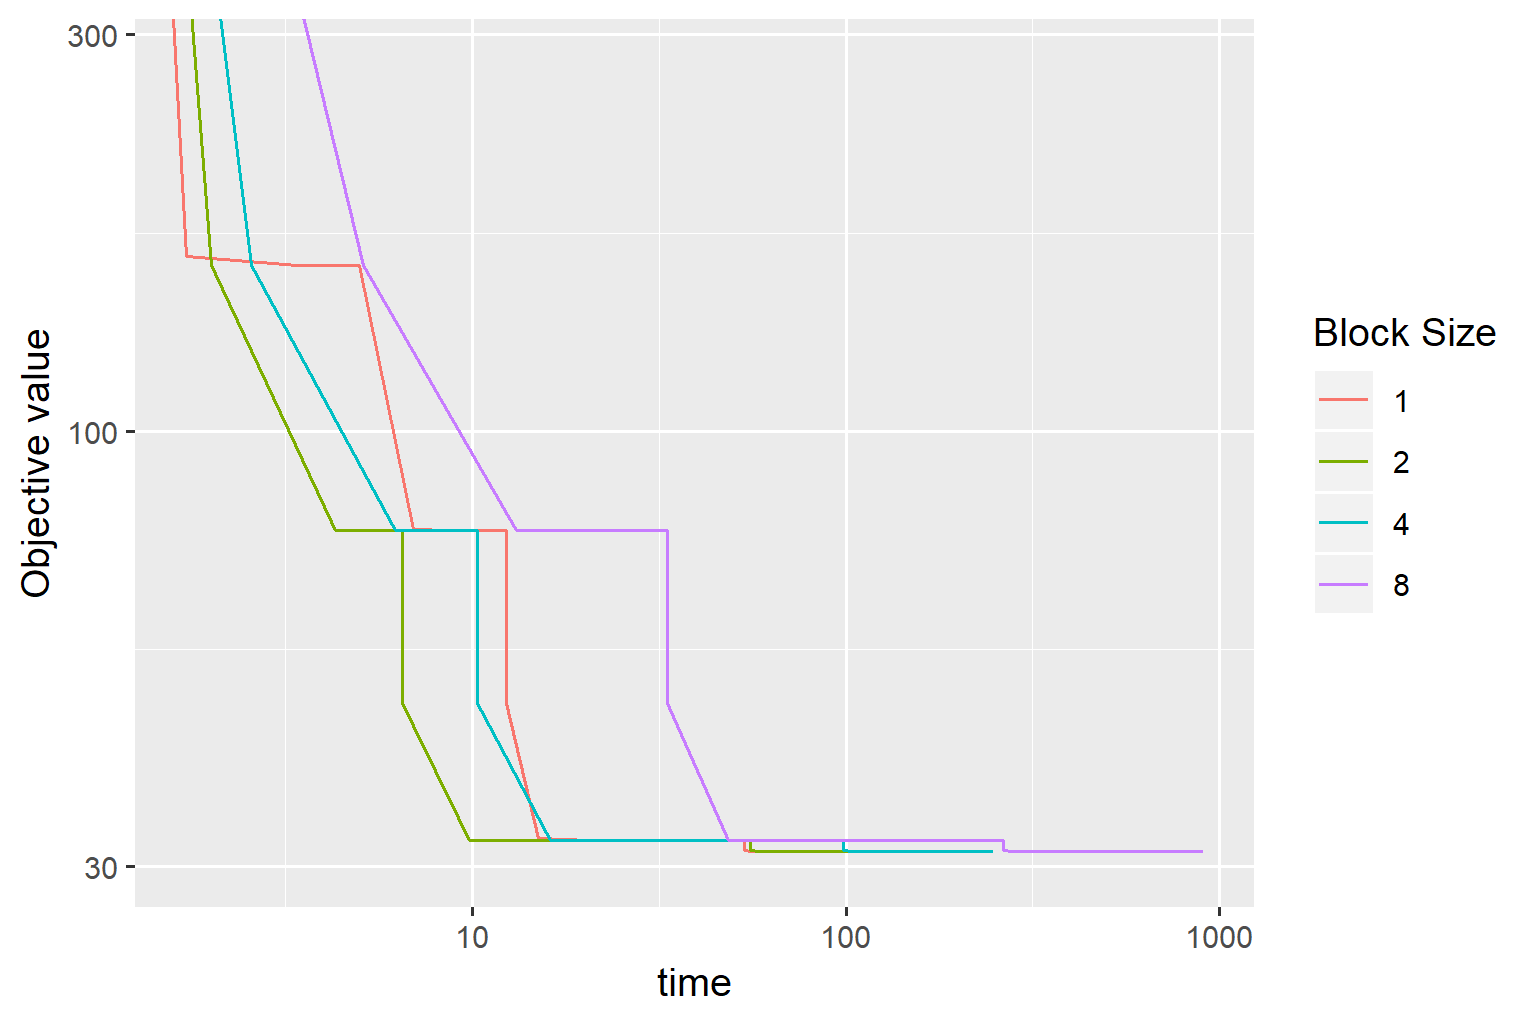
\includegraphics[width=1.0\linewidth]{./chapters/05.pcdm/parameters/blockSize.png}
	\end{subfigure}
	\begin{subfigure}{0.35\linewidth}
		\begin{tabular}{c | c}
			Block Size & Total seconds \\ \hline
			1 & 108 \\
			2 & 103 \\
			4 & 248 \\
			8 & 905 \\
		\end{tabular}
	\end{subfigure}
	\caption{Convergence speedup with $PSF$ approximation}
\end{figure}
Block size is not useful to speed up. More difficult code.

From here on out we will always use single pixels. I.e. blocks of the size of 1.

 

\subsubsection{Pseudo-random strategy}
By how much do we need to search the area.

\begin{figure}[h]
	\centering
	\begin{subfigure}{0.6\linewidth}
		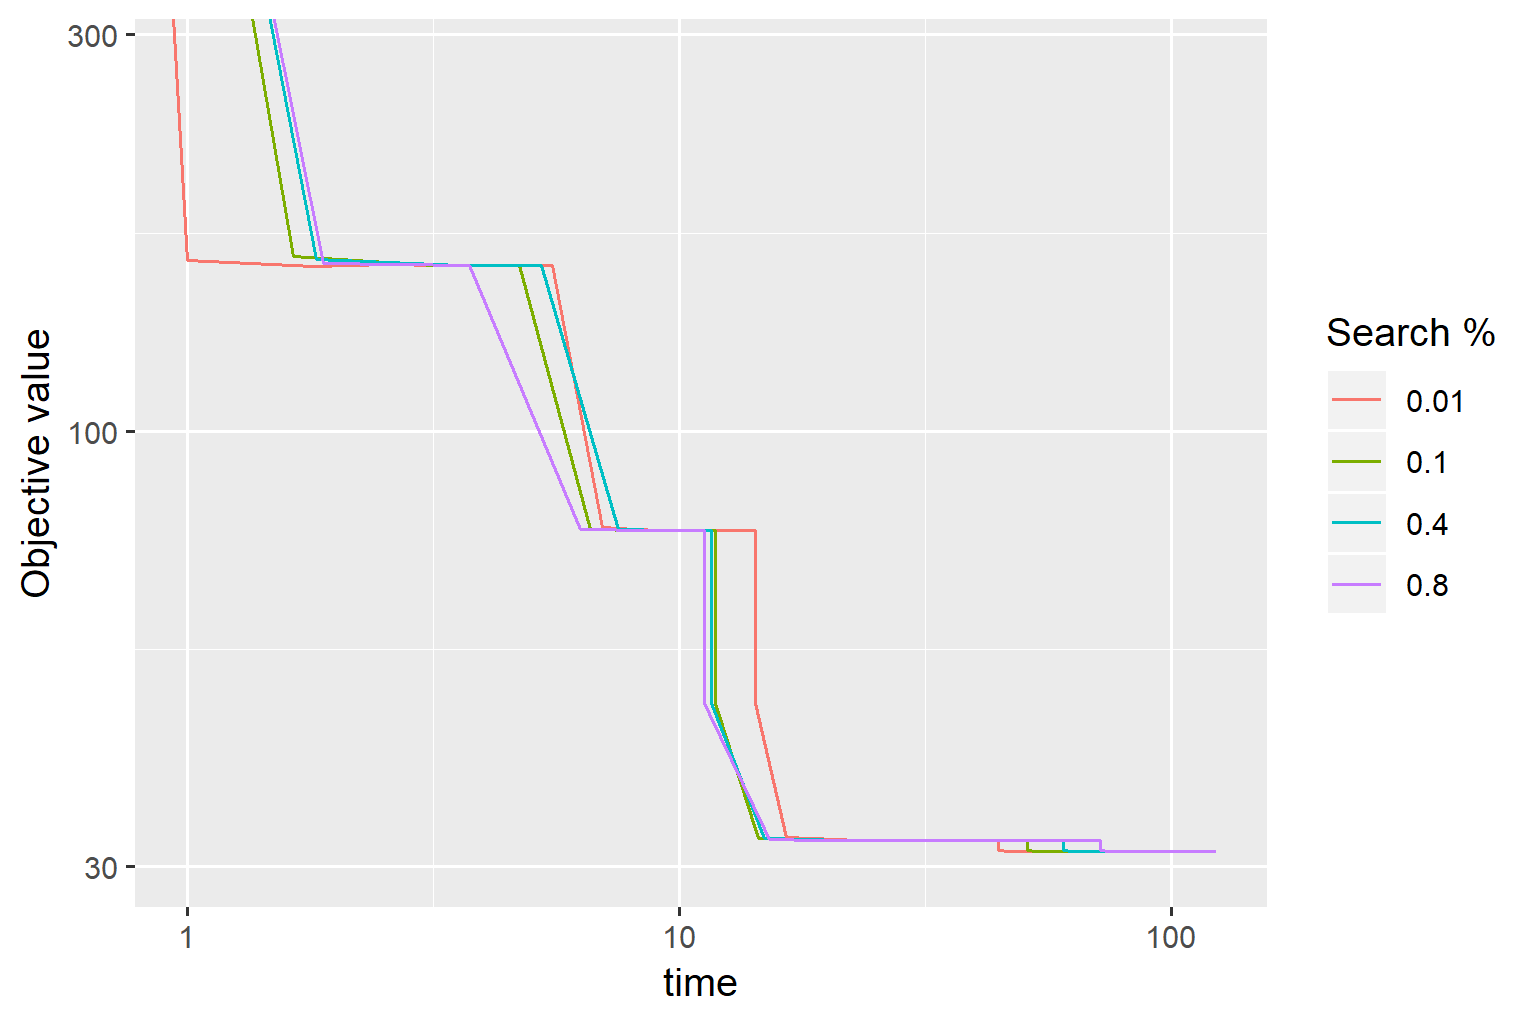
\includegraphics[width=1.0\linewidth]{./chapters/05.pcdm/parameters/searchPercent.png}
	\end{subfigure}
	\begin{subfigure}{0.35\linewidth}
		\begin{tabular}{c | c}
			Search Percentage & Total seconds \\ \hline
			0.01 & 106 \\
			0.1 & 108 \\
			0.2 & 100 \\
			0.4 & 104 \\
			0.8 & 123 \\
		\end{tabular}
	\end{subfigure}
	\caption{Convergence speedup with $PSF$ approximation}
\end{figure}

And it is a tiny fraction. A lot less communication cost. Close to random, but not quite.


\subsubsection{Acceleration}
Not useful

\begin{figure}[h]
	\centering
	\begin{subfigure}{0.6\linewidth}
		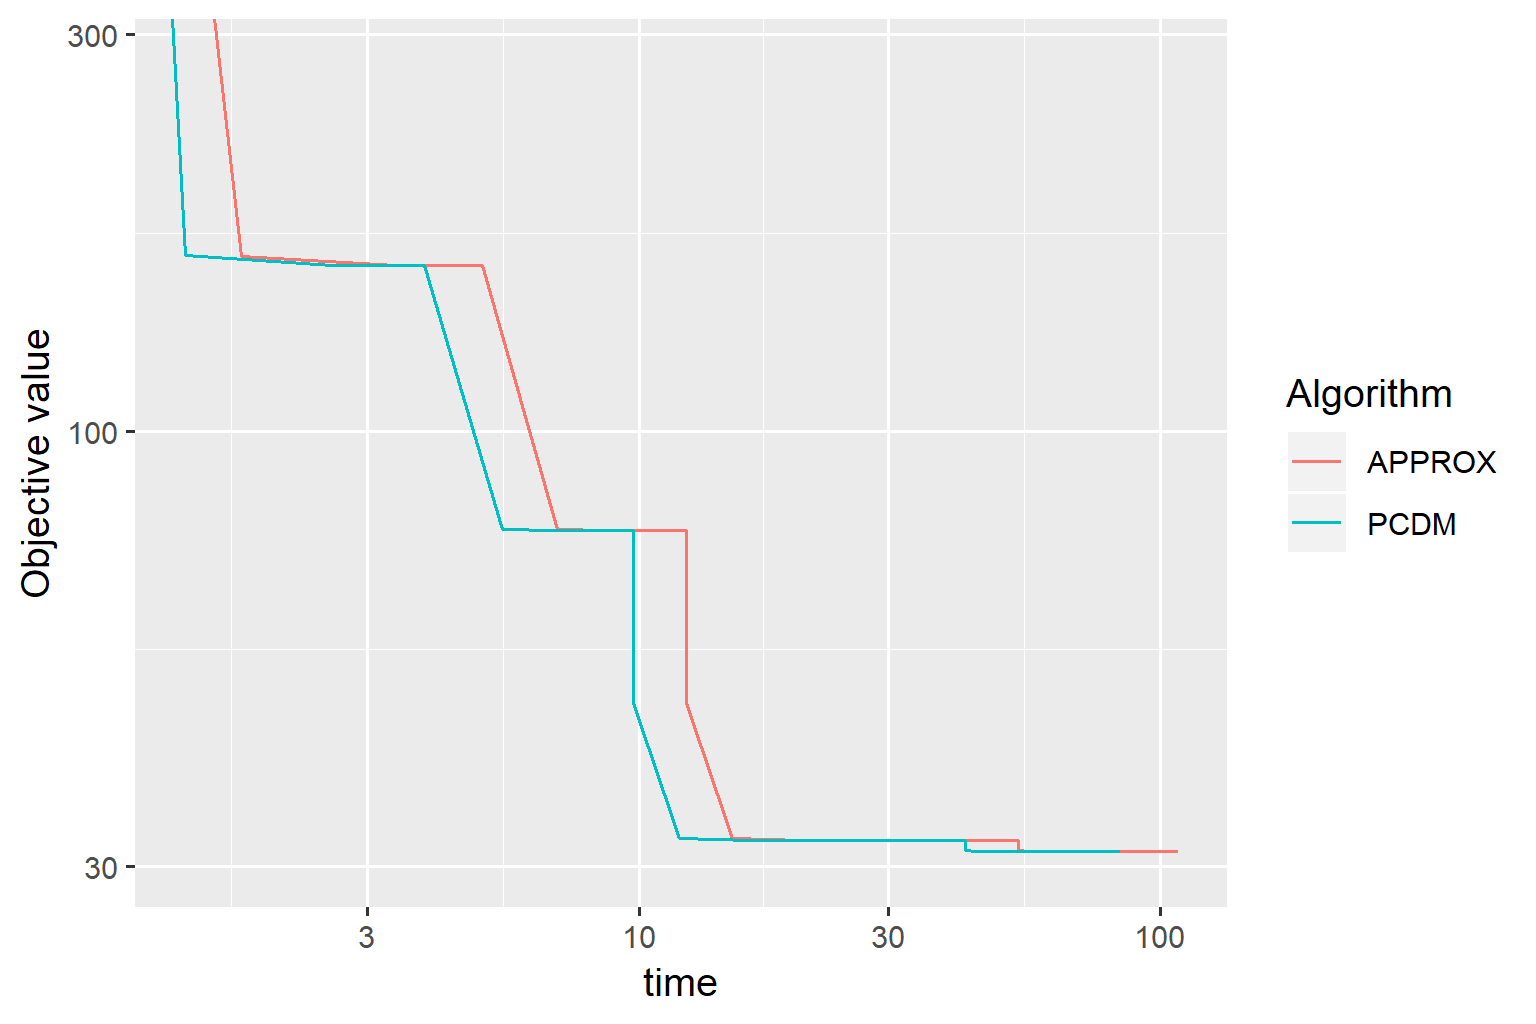
\includegraphics[width=1.0\linewidth]{./chapters/05.pcdm/parameters/acceleration.png}
	\end{subfigure}
	\begin{subfigure}{0.35\linewidth}
		\begin{tabular}{c | c}
			Method & Total seconds \\ \hline
			With Acceleration & 108 \\
			Without Acceleration & 84 \\
		\end{tabular}
	\end{subfigure}
	\caption{Convergence speedup with $PSF$ approximation}
\end{figure}

Acceleration not useful. 
Non-accelerated method is clearly faster at every step. 

aster. Less boilerplate code, meaning it is clearly the better choice


\subsection{Comparison to the serial coordinate descent algorithm}
Which is faster

Proper comparison

Acceleration factor


\subsection{Scalability of the parallel coordinate descent algorithm}
How many processors can we realistically use. At what point does the $ESO$ get too small.




